%%%%%%%%%%%%%%%%%%%%%%%%%%%%%%%%%%%%%%%%%%%%%%%%%%%%%%%%%%%%%%%%%%%%%%%%%%%%%%%
% PREAMBOLO COMUNE PER APPUNTI (Stile Scuro)
%
% Questo file contiene tutte le impostazioni e i pacchetti comuni.
% NON contiene \begin{document} o \end{document}.
%
% Istruzioni per la compilazione del file principale:
% pdflatex -shell-escape nomefile_principale.tex
%%%%%%%%%%%%%%%%%%%%%%%%%%%%%%%%%%%%%%%%%%%%%%%%%%%%%%%%%%%%%%%%%%%%%%%%%%%%%%%

\documentclass{article}

% --- Encoding e lingua ---
\usepackage[utf8]{inputenc}
\usepackage[italian]{babel}

% --- Margini e layout ---
\usepackage{geometry}
\geometry{a4paper, margin=1in}

% --- Font sans-serif (come Helvetica) ---
\usepackage[scaled]{helvet}
\renewcommand{\familydefault}{\sfdefault}
\usepackage[T1]{fontenc}

% --- Matematica ---
\usepackage{amsmath}
\usepackage{amssymb}

% --- Liste personalizzate ---
\usepackage{enumitem}
% \setlist{nosep}

% --- Immagini e Grafica ---
\usepackage{float}
% \usepackage{graphicx}
\usepackage{tikz}
\usetikzlibrary{shapes.geometric, positioning, arrows.meta, calc, fit, backgrounds, patterns, decorations.pathreplacing}

% --- Tabelle Avanzate ---
\usepackage{array}
\usepackage{booktabs}
\usepackage{longtable}

\usepackage{siunitx} % Per unità di misura come GHz, dBm, ecc.

% --- Hyperlink e Metadati PDF ---
\usepackage{hyperref}

\usepackage{graphicx}

\hypersetup{
    colorlinks=true,
    linkcolor=white,
    filecolor=magenta,
    urlcolor=cyan,
    citecolor=green,
    % pdftitle, pdfauthor, ecc. verranno impostati nel file principale
    pdfpagemode=FullScreen,
    bookmarksopen=true,
    bookmarksnumbered=true
}

% --- Licenza del documento ---
\usepackage[
  type={CC},
  modifier={by-sa},
  version={4.0},
]{doclicense}

% --- Colori e Sfondo Nero ---
\usepackage{xcolor}
\pagecolor{black}
\color{white}

% --- Evidenziazione del Codice ---
\usepackage{minted}
\setminted{
    frame=lines,
    framesep=2mm,
    fontsize=\small,
    breaklines=true,
    style=monokai,
    bgcolor=black!80
}
\usemintedstyle{monokai}

% --- Comandi personalizzati per algebra relazionale ---
\newcommand{\Rel}[1]{\textit{#1}} % Per i nomi delle relazioni
\newcommand{\Attr}[1]{\textsf{#1}} % Per i nomi degli attributi

\newcommand{\myunion}{\cup}
\newcommand{\myintersection}{\cap}
\newcommand{\mydifference}{-}
\newcommand{\myrename}[2]{\rho_{#1}(#2)}
\newcommand{\myselectop}[2]{\sigma_{#1}(#2)}
\newcommand{\myproject}[2]{\pi_{#1}(#2)}
\newcommand{\mycartesian}{\times}
\newcommand{\mynaturaljoin}{\bowtie} % Usare \Join da amssymb se disponibile e preferito
\newcommand{\mythetajoin}[3]{#1 \bowtie_{#2} #3} % R1 \bowtie_cond R2

% --- Comandi personalizzati per logica ---
\newcommand{\mylandop}{\wedge}
\newcommand{\myvel}{\vee}
\newcommand{\mynegop}{\neg}
\newcommand{\myforallop}{\forall}
\newcommand{\myexistsop}{\exists}

% --- Join esterni (outer join) ---
% Definizione standard per i join esterni
\def\ojoin{\setbox0=\hbox{$\mynaturaljoin$}%
	\rule[-.02ex]{.25em}{.4pt}\llap{\rule[\ht0]{.25em}{.4pt}}}
\newcommand{\myleftouterjoin}{\mathbin{\ojoin\mkern-5.8mu\mynaturaljoin}}
\newcommand{\myrightouterjoin}{\mathbin{\mynaturaljoin\mkern-5.8mu\ojoin}}
\newcommand{\myfullouterjoin}{\mathbin{\ojoin\mkern-5.8mu\mynaturaljoin\mkern-5.8mu\ojoin}}



% --- Titolo ---
\title{Livello Fisico e Segnali}
\author{Basato sulle slide del Prof. Luciano Bononi}
\date{\today}

\begin{document}

\maketitle
\tableofcontents
\newpage

\section{Background sul Livello Fisico (PHY) Wireless}
Il livello fisico (PHY) si occupa della trasmissione dei bit grezzi attraverso il canale di comunicazione wireless. Comprendere le sue basi è fondamentale per progettare e gestire reti wireless.

\subsection{Proprietà delle Onde Radio (RF - Radio Frequency)}

\subsubsection{Comprensione della Radio Frequenza}
\begin{itemize}
    \item \textbf{Generazione, Copertura e Propagazione:} Le onde RF sono energia elettromagnetica generata da corrente alternata (AC) ad alta frequenza che scorre in un'antenna. L'antenna converte la corrente elettrica ``cablata'' in onde RF e viceversa.
    \item \textbf{Pianificazione Wireless:} La comprensione di come le onde RF si generano e si propagano è cruciale per pianificare la copertura di una rete wireless e gestirla efficacemente.
\end{itemize}
\begin{center}
\begin{tikzpicture}[scale=0.8, every node/.style={transform shape}]
        % Voltaggio
        \begin{scope}[shift={(-2,0)}]
            \draw[->] (0,0) -- (3,0) node[right] {$t$};
            \draw[->] (0,-1) -- (0,1) node[above] {$V$};
            \draw[red, thick] (0,0) sin (0.785,0.8) cos (1.57,-0.8) sin (2.355,0.8) cos (3.14,-0.8);
            \node at (1.5,-1.5) {Voltaggio (AC)};
        \end{scope}
    
        % Antenna (spostata più a destra e migliorata)
        \begin{scope}[shift={(4,0)}]
            % Dipolo verticale (due bracci)
            \draw[thick, themeblue] (4,0.8) -- (4,0.1);  % Braccio superiore
            \draw[thick, themeblue] (4,-0.1) -- (4,-0.8);  % Braccio inferiore
            % Punto di alimentazione (gap e linea di alimentazione)
            \draw[thick, themeblue] (3.7,0) -- (4,0);   % Linea di alimentazione
            \draw[fill=white] (4,0) circle (0.1);  % Punto di alimentazione evidenziato
            \node[right] at (4.3,0) {\small punto di alimentazione};  % Etichetta esplicativa
            \node at (4,-1.5) {Antenna Dipolo};  % Nome più specifico
        
            % Onde RF (migliorate)
            \foreach \i in {1,2,3,4,5} {
                \draw[yellow, opacity=0.9/\i] (4.5+\i*0.25,0) circle (\i*0.5);
            }
            \node at (7,-1.5) {Onde RF};
        \end{scope}
\end{tikzpicture}
\end{center}

\subsubsection{Ampiezza (Amplitude)}
\begin{itemize}
    \item \textbf{Portata:} Segnali RF con ampiezza maggiore (più energia) tendono a propagarsi più lontano.
    \item \textbf{Potenza di Trasmissione (Watts):} È l'energia trasmessa per unità di tempo (Joule/Secondo).
    \[ \text{Potenza } (W) = \text{Tensione } (V) \times \text{Corrente } (A) \]
    Maggiore tensione (energia) muove più elettroni (corrente).
\end{itemize}

\subsubsection{Frequenza (Frequency) e Lunghezza d'Onda (Wavelength)}
\begin{itemize}
    \item \textbf{Spettro Wireless:} L'insieme di tutte le possibili frequenze radio. Solo porzioni di questo spettro sono regolamentate e assegnate a specifiche tecnologie wireless.
    \item \textbf{Relazione:} $\lambda = \frac{c}{f}$
    dove $c$ è la velocità della luce (circa $3 \times 10^8 \, \text{m/s}$) e $f$ è la frequenza in Hertz (Hz).
    \item \textbf{Esempio Pratico (Banda ISM a \SI{2.4}{\giga\hertz}):}
    $f = \SI{2.4}{\giga\hertz} = 2.4 \times 10^9 \, \text{Hz}$
    \[ \lambda = \frac{3 \times 10^8 \, \text{m/s}}{2.4 \times 10^9 \, \text{Hz}} = 0.125 \, \text{m} = \SI{12.5}{\centi\meter} \]
    \item \textbf{Importanza Pratica per le Antenne:} Le antenne funzionano meglio quando la loro dimensione fisica è un multiplo o sottomultiplo della lunghezza d'onda (es. $1, \frac{1}{2}, \frac{1}{4}$ di $\lambda$).
\end{itemize}
\begin{center}
\begin{tikzpicture}[scale=0.9, every node/.style={transform shape}]
    \draw[->] (0,0) -- (5,0) node[right] {Tempo (s)};
    \draw[->] (0,-1.2) -- (0,2.2) node[above] {f};
    % Alta frequenza
    \draw[themeblue, thick] (0.5,1.5) sin (0.75,1.8) cos (1.0,1.2) sin (1.25,1.8) cos (1.5,1.2) sin (1.75,1.8) cos (2.0,1.2) sin (2.25,1.8) cos (2.5,1.2) sin (2.75,1.8) cos (3.0,1.2);
    \node[themeblue] at (1.75,2.2) {Alte Frequenze};
    % Bassa frequenza
    \draw[red, thick] (0.5,0) sin (1.5,0.5) cos (2.5,-0.5) sin (3.5,0.5) cos (4.5,-0.5);
    \node[red] at (2.5,-0.9) {Basse Frequenze};
\end{tikzpicture}
\end{center}

\subsubsection{Fase (Phase)}
\begin{itemize}
    \item \textbf{Definizione:} Sfasamento dell'onda rispetto a un punto di riferimento (gradi o radianti).
    \begin{itemize}
        \item Fase Positiva (left-shift): fronte d'onda anticipato.
        \item Fase Negativa (right-shift): fronte d'onda ritardato.
    \end{itemize}
    \item \textbf{Effetti Pratici (Eco e Interferenza):} Segnali riflessi (echi) arrivano con fasi diverse.
    \begin{itemize}
        \item Se \textbf{in fase}: interferenza costruttiva (segnale più forte).
        \item Se \textbf{in controfase} (sfasate di \SI{180}{\degree}): interferenza distruttiva (segnale più debole o nullo).
    \end{itemize}
\end{itemize}
\begin{center}
    \begin{tikzpicture}[scale=0.9, every node/.style={transform shape}]
        % Axes
        \draw[->] (0,0) -- (7,0) node[right] {Tempo/Fase (gradi)};
        \draw[->] (0,-1.5) -- (0,1.5) node[above] {Ampiezza};
        
        % Reference dashed line
        \draw[dashed, gray] (0,1) -- (6.5,1);
        
        % Signal plots
        % Main signal (phase 0) - themeblue
        \draw[thick, themeblue] plot[domain=0:6.28, samples=100] (\x, {sin(\x r)});
        
        % Phase +90° signal - red
        \draw[thick, red] plot[domain=0:6.28, samples=100] (\x, {sin((\x+1.57) r)*0.5});
        
        % Phase +180° signal - green
        \draw[thick, green] plot[domain=0:6.28, samples=100] (\x, {sin((\x+3.14) r)*0.7});
        
        % Legend in top right corner
        \node[anchor=north east] at (11,2.2) {
            \begin{tabular}{ll}
                \textcolor{themeblue}{---} & Segnale (fase 0) \\
                \textcolor{red}{---} & Segnale (fase +90°) \\
                \textcolor{green}{---} & Segnale (fase +180°)
            \end{tabular}
        };
    \end{tikzpicture}
\end{center}

\subsubsection{Polarizzazione (Polarization)}
\begin{itemize}
    \item \textbf{Definizione:} Orientamento fisico dell'antenna, che determina l'orientamento del campo elettrico dell'onda RF.
    \item \textbf{Componenti Onda RF:} Campo Elettrico (E-field) e Campo Magnetico (H-field), perpendicolari tra loro.
    \item \textbf{Tipi Comuni:}
    \begin{itemize}
        \item Polarizzazione Orizzontale: Campo elettrico parallelo al suolo.
        \item Polarizzazione Verticale: Campo elettrico perpendicolare al suolo (comune nelle WLAN).
    \end{itemize}
    \item \textbf{Importanza Pratica:} Per comunicazione ottimale, le antenne trasmittente e ricevente dovrebbero avere la \textbf{stessa polarizzazione}. Disallineamenti causano perdita di segnale.
\end{itemize}
\begin{center}
\begin{tikzpicture}[scale=0.7, every node/.style={transform shape}]
    % Polarizzazione Verticale
    \node at (-2, 2.5) {Polarizzazione Verticale};
    \draw[thick] (-2,0) -- (-2,2); % Antenna
    \foreach \i in {0.2,0.4,...,1.8} {
        \draw[themeblue, ->] (-2,\i) -- (-1.5,\i); % Campo Elettrico
    }
    \draw[dashed] (-3,-0.5) -- (0,-0.5) node[right] {Suolo};
    % Stickman
    \draw (-2.5, -0.5) -- (-2.5, 0.5) -- (-2.2, 0.2) -- (-2.5, 0.5) -- (-2.8, 0.2);
    \draw (-2.5,0.5) circle (0.2);


    % Polarizzazione Orizzontale
    \node at (3.5, 2.5) {Polarizzazione Orizzontale};
    \draw[thick] (2.5,1) -- (4.5,1); % Antenna
     \foreach \i in {2.7,2.9,...,4.3} {
        \draw[themeblue, ->] (\i,1) -- (\i,1.5); % Campo Elettrico (verso alto per visibilità)
    }
    \draw[dashed] (2,-0.5) -- (5,-0.5) node[right] {Suolo};
    % Stickman
    \draw (3.5, -0.5) -- (3.5, 0.5) -- (3.8, 0.2) -- (3.5, 0.5) -- (3.2, 0.2);
    \draw (3.5,0.5) circle (0.2);
\end{tikzpicture}
\end{center}
\textbf{N.B.:} Il problema della polarizzazione è molto importante per lunghe distanze e antenne direzionali. A breve distanza, le riflessioni mitigano il disallineamento.

\section{Propagazione RF e Comportamenti}

\subsection{Copertura della Trasmissione Radio}
\begin{itemize}
    \item \textbf{Attenuazione con la Distanza:} La potenza del segnale (P) diminuisce con $P \propto \frac{P_{tx}}{d^k}$ (dove $\propto$ significa ``proporzionale a'', $P_{tx}$ è la potenza di trasmissione iniziale e $d^k$ è la distanza elevata all'esponente $k$).
    \begin{itemize}
        \item In spazio libero, $k \approx 2$.
        \item Con ostacoli, $k \ge 3$.
    \end{itemize}
    \item \textbf{Effetto della Potenza di Trasmissione $P_{tx}$:} Aumentando $P_{tx}$, il segnale arriva più lontano.
\end{itemize}

\begin{center}
\begin{tikzpicture}[scale=0.9, every node/.style={transform shape}]
    % Sorgente
    \node[draw, circle, fill=themeblue!30, minimum size=8mm, text=black] (A) at (0,0) {A};
    
    % Onde radio con intensità decrescente
    \draw[themeblue, very thick, opacity=0.9] (A) circle (0.8cm);
    \draw[themeblue, thick, opacity=0.7] (A) circle (1.4cm);
    \draw[themeblue, opacity=0.5] (A) circle (2.0cm);
    \draw[themeblue, opacity=0.3] (A) circle (2.6cm);
    
    % Frecce per indicare la propagazione
    \draw[->, themeblue, thick] (0.6,0.6) -- (1.2,1.2);
    \draw[->, themeblue, thick] (0.6,-0.6) -- (1.2,-1.2);
    \draw[->, themeblue, thick] (-0.6,0.6) -- (-1.2,1.2);
    \draw[->, themeblue, thick] (-0.6,-0.6) -- (-1.2,-1.2);
    
    % Etichette per le zone (più in alto e a destra)
    \node[themeblue, font=\tiny] at (0.85,0.55) {\textbf{Alta}};
    \node[themeblue, font=\tiny] at (1.5,0.75) {\textbf{Media}};
    \node[themeblue, font=\tiny] at (2.07,0.95) {\textbf{Bassa}};
    \node[themeblue, font=\tiny] at (2.9,1.15) {\textbf{Molto bassa}};
    
    % Grafico attenuazione con miglioramenti
    \begin{scope}[xshift=5.5cm, yshift=-3cm]
        \draw[->] (0,0) -- (4.5,0) node[right] {\textbf{Distanza (d)}};
        \draw[->] (0,0) -- (0,6) node[above] {\textbf{Potenza Ricevuta}};
        
        % Curve per diverse potenze di trasmissione (senza etichette)
        \draw[red, very thick] plot[smooth, domain=0.5:4] (\x, {2.8/\x});
        \draw[orange, thick] plot[smooth, domain=0.5:4] (\x, {2.0/\x});
        \draw[themeblue, thick] plot[smooth, domain=0.5:4] (\x, {1.4/\x});
        
        % Legenda in alto a destra
        \node[draw, align=left, font=\small] at (3.5,5) {
            \textcolor{red}{— $P_{tx} = 4W$}\\
            \textcolor{orange}{— $P_{tx} = 2W$}\\
            \textcolor{themeblue}{— $P_{tx} = 1W$}
        };
        
        % Limite di rilevamento
        \draw[primarytext, dashed, thick] (0,0.3) -- (4,0.3) node[right, font=\small] {Limite rilevamento};
        
        % Punti di intersezione per mostrare il range (corretti)
        \fill[red] (3.8,0.3) circle (2pt);
        \fill[orange] (2.6,0.3) circle (2pt);
        \fill[themeblue] (1.8,0.3) circle (2pt);
        
        % Linee verticali per mostrare il range massimo (corrette)
        \draw[red, dotted] (3.8,0) -- (3.8,0.3);
        \draw[orange, dotted] (2.6,0) -- (2.6,0.3);
        \draw[themeblue, dotted] (1.8,0) -- (1.8,0.3);
        
        % Etichette per i range (dentro il grafico)
        \node[red, font=\small] at (3.8,-0.2) {R$_{max}$};
        \node[orange, font=\small] at (2.6,-0.2) {R$_{med}$};
        \node[themeblue, font=\small] at (1.8,-0.2) {R$_{min}$};
    \end{scope}
\end{tikzpicture}
\end{center}

\vspace{0.3cm}
\textbf{Spiegazione dei grafici:}
\begin{itemize}
    \item \textbf{Grafico a sinistra (Propagazione):} Mostra come le onde radio si propagano dalla sorgente A in tutte le direzioni. I cerchi rappresentano zone con diversa intensità del segnale: più ci si allontana dalla sorgente, più il segnale diventa debole.
    
    \item \textbf{Grafico a destra (Attenuazione):} Mostra come la potenza ricevuta diminuisce con la distanza per diverse potenze di trasmissione. Il punto dove ogni curva interseca la linea tratteggiata rappresenta il range massimo di comunicazione per quella potenza.
\end{itemize}

\subsection{Portate (Ranges) della Propagazione del Segnale Wireless}
\begin{itemize}
    \item \textbf{Transmission Range:} Comunicazione possibile con basso tasso di errore.
    \item \textbf{Detection Range:} Segnale rilevabile, ma comunicazione non affidabile.
    \item \textbf{Interference Range:} Segnale abbastanza forte da interferire, anche se non rilevabile.
\end{itemize}
\textbf{Importante:} Queste portate \textbf{dipendono dalla sensibilità del ricevitore!}
\begin{center}
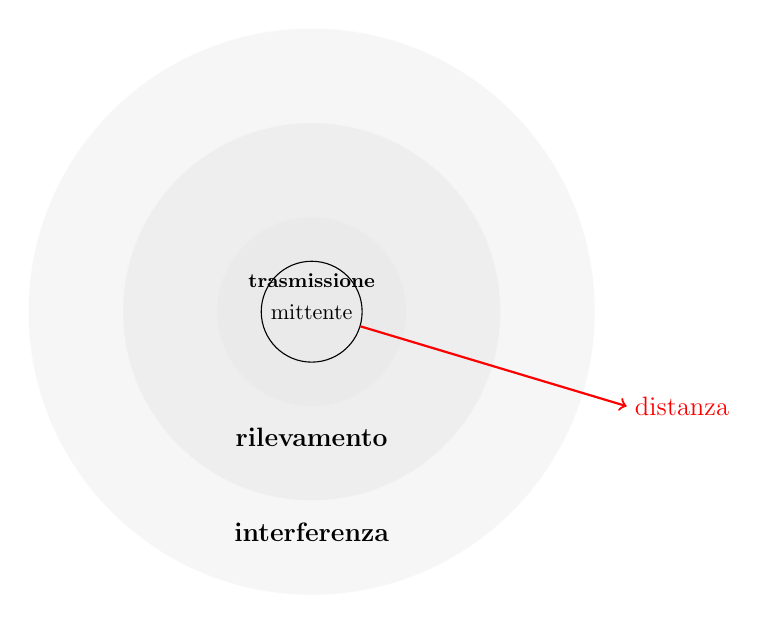
\begin{tikzpicture}[scale=0.8, every node/.style={transform shape}]
    % First draw all the circles with opacity
    \draw[fill=gray!50, draw=white, opacity=0.7] (0,0) circle (1.5cm);
    \draw[fill=gray!30, draw=white, opacity=0.7] (0,0) circle (3cm);
    \draw[fill=gray!10, draw=white, opacity=0.7] (0,0) circle (4.5cm);
    
    % Then add all text nodes without opacity
    \node[draw, circle, text=black] (sender) at (0,0) {mittente};
    \node[text=black, font=\bfseries\small] at (0,0.5cm) {trasmissione};
    \node[text=black, font=\bfseries\large] at (0,-2cm) {rilevamento};
    \node[text=black, font=\bfseries\large] at (0,-3.5cm) {interferenza};
    \draw[->, thick, red] (sender) -- (5, -1.5) node[right, text=red, font=\large] {distanza};
\end{tikzpicture}
\end{center}

\subsection{Effetto degli Ostacoli}
Gli ostacoli possono \textbf{riflettere} o \textbf{assorbire} le onde RF. L'effetto dipende dal materiale e dalla frequenza.
\begin{itemize}
    \item \textbf{Alte Frequenze (es. \SI{5}{\giga\hertz}, \SI{6}{\giga\hertz}):} Più attenuate dagli ostacoli, migliori per brevi distanze.
    \item \textbf{Basse Frequenze (es. \SI{900}{\mega\hertz}):} Penetrano meglio gli ostacoli, migliori per lunghe distanze.
\end{itemize}

\subsection{Effetti della Propagazione del Segnale Wireless}
\begin{itemize}
    \item \textbf{Fading:} Fluttuazioni della potenza del segnale.
    \item \textbf{Shadowing:} Attenuazione da grossi ostacoli.
    \item \textbf{Reflection (Riflessione):} Rimbalzo su grandi superfici.
    \item \textbf{Refraction (Rifrazione):} Cambio direzione attraverso mezzi diversi.
    \item \textbf{Scattering (Diffusione):} Dispersione da piccoli ostacoli.
    \item \textbf{Diffraction (Diffrazione):} Piegamento attorno ai bordi.
\end{itemize}

% Grid layout for propagation effects
\begin{center}
\begin{minipage}[t]{0.48\textwidth}
    \centering
    % 1. REFLECTION (Riflessione)
    \begin{tikzpicture}[scale=0.9]
        \node at (0,3.5) {\textbf{Reflection (Riflessione)}};
        
        % Transmitter
        \fill[red!70] (0,0) circle (0.1);
        \node[below] at (0,-0.2) {TX};
        
        % Receiver
        \fill[blue!70] (4,2) circle (0.1);
        \node[above] at (4,2.2) {RX};
        
        % Edificio/Wall
        \fill[gray!60] (2,-0.5) rectangle (2.5,3);
        \node[rotate=90] at (2.25,1.2) {Edificio};
        
        % Direct path (blocked)
        \draw[red, dashed, thick] (0,0) -- (1.8,1.5);
        \draw[red, thick, cross out, draw=red] (1.9,1.6) circle (0.1);
        
        % Reflected path
        \draw[->, red, thick] (0,0) -- (2,2.5);
        \draw[->, red, thick] (2,2.5) -- (4,2);
        
        % Reflection point
        \fill[green!70] (2,2.5) circle (0.05);
        
        % Angle indicators
        \draw[thin] (1.8,2.5) -- (2.2,2.5);
        \draw[thin] (2,2.3) -- (2,2.7);
        \node[font=\small] at (1.7,2.2) {$\theta_i$};
        \node[font=\small] at (2.3,2.2) {$\theta_r$};
        
        \node[below] at (2,-0.7) {$\theta_i = \theta_r$};
    \end{tikzpicture}
\end{minipage}
\hfill
\begin{minipage}[t]{0.48\textwidth}
    \centering
    % 2. DIFFRACTION (Diffrazione)
    \begin{tikzpicture}[scale=0.9]
        \node at (0,3.5) {\textbf{Diffraction (Diffrazione)}};
        
        % Transmitter
        \fill[red!70] (0,1) circle (0.1);
        \node[below] at (0,0.8) {TX};
        
        % Receiver
        \fill[blue!70] (4,1) circle (0.1);
        \node[below] at (4,0.8) {RX};
        
        % Obstacle (building)
        \fill[gray!60] (1.5,0) rectangle (2.5,2.5);
        \node[rotate=90] at (2,1.2) {Edificio};
        
        % Direct path (blocked)
        \draw[red, dashed, thick] (0,1) -- (1.4,1);
        \draw[red, thick, cross out, draw=red] (1.5,1) circle (0.1);
        
        % Diffracted waves around top edge
        \draw[->, red, thick] (0,1) -- (2,2.5);
        \draw[->, red, thick, bend left=20] (2,2.5) to (4,1);
        
        % Additional diffracted rays
        \draw[->, red!60, thick, bend left=30] (2,2.5) to (3.5,0.5);
        \draw[->, red!60, thick, bend left=10] (2,2.5) to (3.5,1.5);
        
        % Edge point
        \fill[green!70] (2,2.5) circle (0.05);
        \node[right, font=\small] at (2.1,2.5) {Angolo};
        
        % Shadow region
        \fill[black!30, opacity=0.4] (2.5,0) rectangle (4,2);
        \node[font=\small] at (3.2,-0.4) {Shadow Region};
    \end{tikzpicture}
\end{minipage}

\vspace{1cm}

\begin{minipage}[t]{0.48\textwidth}
    \centering
    % 3. SCATTERING (Diffusione)
    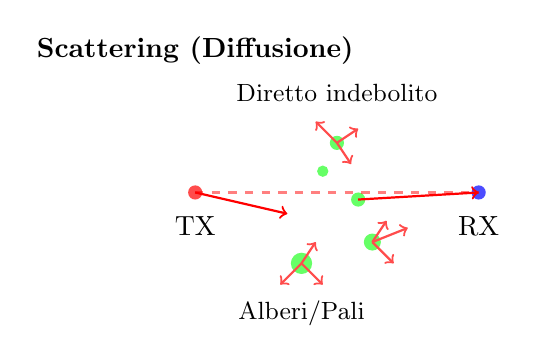
\begin{tikzpicture}[scale=0.9]
        \node at (0,3.5) {\textbf{Scattering (Diffusione)}};
        
        % Transmitter
        \fill[red!70] (0,1.5) circle (0.1);
        \node[below] at (0,1.3) {TX};
        
        % Receiver
        \fill[blue!70] (4,1.5) circle (0.1);
        \node[below] at (4,1.3) {RX};
        
        % Small obstacles (trees, poles, etc.)
        \fill[green!60] (1.5,0.5) circle (0.15);
        \fill[green!60] (2,2.2) circle (0.1);
        \fill[green!60] (2.5,0.8) circle (0.12);
        \fill[green!60] (1.8,1.8) circle (0.08);
        \fill[green!60] (2.3,1.4) circle (0.1);
        
        \node[font=\small] at (1.5,-0.2) {Alberi/Pali};
        
        % Incident wave
        \draw[->, red, thick] (0,1.5) -- (1.3,1.2);
        
        % Scattered waves in multiple directions
        \draw[->, red!70, thick] (1.5,0.5) -- (1.2,0.2);
        \draw[->, red!70, thick] (1.5,0.5) -- (1.8,0.2);
        \draw[->, red!70, thick] (1.5,0.5) -- (1.7,0.8);
        
        \draw[->, red!70, thick] (2,2.2) -- (1.7,2.5);
        \draw[->, red!70, thick] (2,2.2) -- (2.3,2.4);
        \draw[->, red!70, thick] (2,2.2) -- (2.2,1.9);
        
        \draw[->, red!70, thick] (2.5,0.8) -- (2.8,0.5);
        \draw[->, red!70, thick] (2.5,0.8) -- (2.7,1.1);
        \draw[->, red!70, thick] (2.5,0.8) -- (3,1);
        
        % One scattered ray reaching receiver
        \draw[->, red, thick] (2.3,1.4) -- (4,1.5);
        
        % Direct path (weakened)
        \draw[red, dashed, thick, opacity=0.5] (0,1.5) -- (4,1.5);
        \node[font=\small] at (2,2.9) {Diretto indebolito};
    \end{tikzpicture}
\end{minipage}
\hfill
\begin{minipage}[t]{0.48\textwidth}
    \centering
    % 4. MULTIPATH FADING
    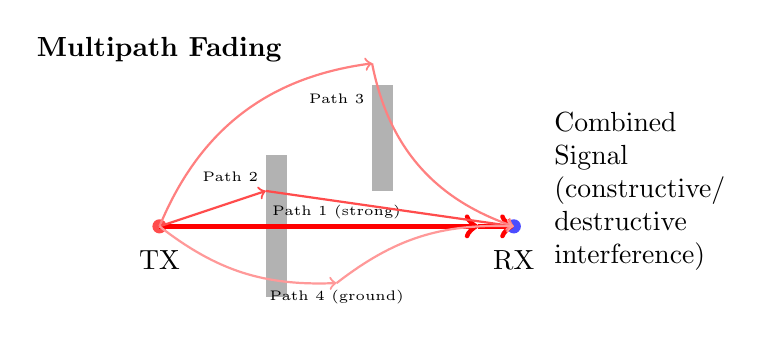
\begin{tikzpicture}[scale=0.9]
        \node at (0,3.5) {\textbf{Multipath Fading}};
        
        % Transmitter
        \fill[red!70] (0,1) circle (0.1);
        \node[below] at (0,0.8) {TX};
        
        % Receiver
        \fill[blue!70] (5,1) circle (0.1);
        \node[below] at (5,0.8) {RX};
        
        % Obstacles
        \fill[gray!60] (1.5,0) rectangle (1.8,2);
        \fill[gray!60] (3,1.5) rectangle (3.3,3);
        
        % Multiple paths with different delays and amplitudes
        % Path 1 - Direct (strongest but partially blocked)
        \draw[->, red, thick, line width=2pt] (0,1) -- (4.5,1);
        \draw[->, red, thick, line width=2pt] (4.5,1) -- (5,1);
        \node[font=\tiny] at (2.5,1.2) {Path 1 (strong)};
        
        % Path 2 - Reflected from building
        \draw[->, red!70, thick] (0,1) -- (1.5,1.5);
        \draw[->, red!70, thick] (1.5,1.5) -- (5,1);
        \node[font=\tiny] at (1,1.7) {Path 2};
        
        % Path 3 - Over building
        \draw[->, red!50, thick, bend left=30] (0,1) to (3,3.3);
        \draw[->, red!50, thick, bend right=30] (3,3.3) to (5,1);
        \node[font=\tiny] at (2.5,2.8) {Path 3};
        
        % Path 4 - Ground reflection
        \draw[->, red!40, thick, bend right=20] (0,1) to (2.5,0.2);
        \draw[->, red!40, thick, bend left=20] (2.5,0.2) to (5,1);
        \node[font=\tiny] at (2.5,0) {Path 4 (ground)};
        
        % Signal combination at receiver
        \node[right] at (5.2,1.5) {\begin{tabular}{l}
            Combined\\
            Signal\\
            (constructive/\\
            destructive\\
            interference)
        \end{tabular}};
    \end{tikzpicture}
\end{minipage}

\vspace{1cm}

\begin{minipage}[t]{0.48\textwidth}
    \centering
    % 5. SHADOWING
    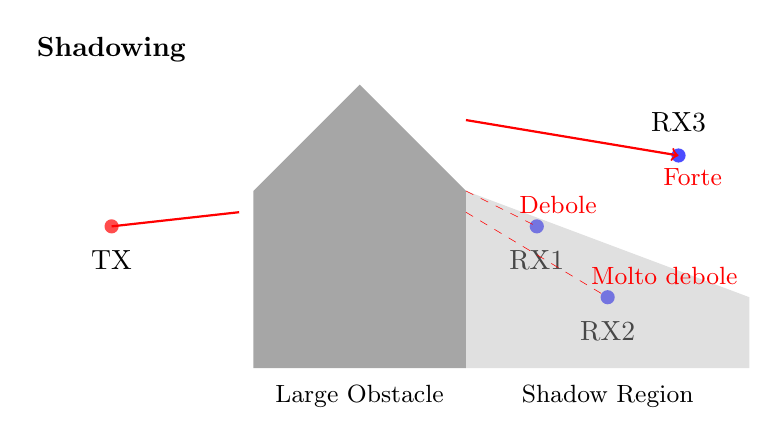
\begin{tikzpicture}[scale=0.9]
        \node at (0,4.5) {\textbf{Shadowing}};
        
        % Transmitter
        \fill[red!70] (0,2) circle (0.1);
        \node[below] at (0,1.8) {TX};
        
        % Large obstacle (mountain/large building)
        \fill[gray!70] (2,0) -- (2,2.5) -- (3.5,4) -- (5,2.5) -- (5,0) -- cycle;
        \node[font=\small] at (3.5,-0.4) {Large Obstacle};
        
        % Receivers at different positions
        \fill[blue!70] (6,2) circle (0.1);
        \node[below] at (6,1.8) {RX1};
        \fill[blue!70] (7,1) circle (0.1);
        \node[below] at (7,0.8) {RX2};
        \fill[blue!70] (8,3) circle (0.1);
        \node[above] at (8,3.2) {RX3};
        
        % Signal strength visualization
        \draw[red, thick] (0,2) -- (1.8,2.2);
        
        % Shadow region
        \fill[black!30, opacity=0.4] (5,0) -- (5,2.5) -- (9,1) -- (9,0) -- cycle;
        \node[font=\small] at (7,-0.4) {Shadow Region};
        
        % Weak signals in shadow
        \draw[red, dashed, very thin] (5,2.5) -- (6,2);
        \draw[red, dashed, very thin] (5,2.2) -- (7,1);
        
        % Strong signal outside shadow
        \draw[->, red, thick] (5,3.5) -- (8,3);
        
        % Signal strength indicators
        \node[font=\small, red] at (6.3,2.3) {Debole};
        \node[font=\small, red] at (7.8,1.3) {Molto debole};
        \node[font=\small, red] at (8.2,2.7) {Forte};
    \end{tikzpicture}
\end{minipage}
\end{center}

\subsection{Propagazione Multipath (Percorsi Multipli)}
Il segnale raggiunge il ricevitore tramite percorsi multipli.
\begin{itemize}
    \item \textbf{Time Dispersion (Dispersione Temporale):} Copie del segnale arrivano in istanti diversi.
    \begin{itemize}
        \item \textbf{Inter-Symbol Interference (ISI):} Sovrapposizione di simboli, causa errori.
    \end{itemize}
    \item \textbf{Distorsione del Segnale:} Il segnale risultante è la somma di copie con fasi e ampiezze diverse.
\end{itemize}

\subsection{Effetti della Mobilità}
Il movimento cambia le caratteristiche del canale.
\begin{itemize}
    \item \textbf{Fading a Breve Termine (Short Term Fading):} Rapide fluttuazioni di potenza.
    \item \textbf{Fading a Lungo Termine (Long Term Fading):} Cambiamenti lenti nella potenza media.
\end{itemize}

\subsection{Voltage Standing Wave Ratio (VSWR)}
\subsubsection{Cos'è il VSWR?}
Il VSWR è un fenomeno che si verifica nei sistemi di trasmissione RF quando c'è un "disadattamento di impedenza" tra i vari componenti.

Con un'analogia, si può immaginare un tubo dell'acqua (il cavo) che collega una pompa (il trasmettitore) a un irrigatore (l'antenna):
\begin{itemize}
    \item Se il tubo ha lo stesso diametro ovunque, l'acqua scorre senza problemi
    \item Se improvvisamente il tubo cambia diametro, parte dell'acqua "rimbalza" indietro, creando turbolenze
\end{itemize}

Allo stesso modo, nelle trasmissioni RF:
\begin{itemize}
    \item L'impedenza (misurata in Ohm $\Omega$) è come il "diametro del tubo" per i segnali RF
    \item Se tutti i componenti hanno la stessa impedenza, il segnale viaggia senza problemi
    \item Se c'è un cambio di impedenza, parte del segnale viene riflesso indietro
\end{itemize}

\subsubsection{Problemi del VSWR}
\begin{itemize}
    \item \textbf{Causa:} Discrepanza di impedenza ($\Omega$) tra trasmettitore, cavo, antenna
    \item \textbf{Effetto (``Return Loss''):} 
    \begin{itemize}
        \item Parte dell'energia viene riflessa indietro verso il trasmettitore
        \item Si creano "onde stazionarie" nel cavo (da qui il nome "Standing Wave")
        \item Meno potenza raggiunge effettivamente l'antenna
    \end{itemize}
    \item \textbf{Conseguenze Negative:} 
    \begin{itemize}
        \item Danneggiamento del trasmettitore (l'energia riflessa può surriscaldarlo)
        \item Instabilità del segnale
        \item Perdita di potenza effettiva trasmessa
        \item Distorsione del segnale
    \end{itemize}
\end{itemize}

\subsubsection{Come si Misura}
\begin{itemize}
    \item Il VSWR è un rapporto tra impedenze, espresso come X:1
    \item VSWR = 1:1 è il caso ideale (nessuna riflessione)
    \item VSWR = 2:1 significa che circa l'11\% della potenza viene riflessa
    \item VSWR = 3:1 significa che circa il 25\% della potenza viene riflessa
\end{itemize}

\subsubsection{Soluzioni}
\begin{itemize}
    \item \textbf{Soluzione Principale:} Usare componenti con la \textbf{stessa impedenza}
    \begin{itemize}
        \item Nelle WLAN moderne si usa tipicamente un'impedenza di \SI{50}{\ohm}
        \item Tutti i componenti (Tx, cavi, antenna) devono essere \SI{50}{\ohm}
    \end{itemize}
    \item \textbf{Alternative:}
    \begin{itemize}
        \item Usare "adattatori di impedenza" tra componenti diversi
        \item Scegliere cavi di alta qualità con impedenza controllata
        \item Minimizzare le giunzioni e i connettori non necessari
    \end{itemize}
\end{itemize}

\begin{center}
    \begin{tikzpicture}[scale=1.2, every node/.style={transform shape}]
        % Trasmettitore
        \node (tx) [draw, rectangle, fill=blue!30, minimum height=1.2cm, minimum width=2.5cm, 
                    text width=2cm, align=center, text=black] at (0,0) {Trasmettitore\\$Z_{out} = \SI{75}{\ohm}$};
        
        % Primo cavo
        \node (cable1) [draw, rectangle, fill=green!30, minimum height=0.8cm, minimum width=2.5cm,
                        text width=2cm, align=center, text=black] at (4,0) {Cavo\\$Z_c = \SI{75}{\ohm}$};
        
        % Secondo cavo
        \node (cable2) [draw, rectangle, fill=red!30, minimum height=0.8cm, minimum width=2.5cm,
                        text width=2cm, align=center, text=black] at (8,0) {Cavo\\$Z_c = \SI{50}{\ohm}$};
        
        % Antenna
        \node (ant) [trapezium, draw, fill=yellow!30, minimum height=1.2cm, minimum width=2cm,
                     shape border rotate=270, text width=1.8cm, align=center, text=black] at (11.5,0) {Antenna\\$Z_L = \SI{50}{\ohm}$};
    
        % Connessioni
        \draw[->, thick] (tx.east) -- (cable1.west);
        \draw[->, thick] (cable1.east) -- (cable2.west);
        \draw[->, thick] (cable2.east) -- (ant.west);
        
        % Etichette VSWR
        \node[above, font=\small\bfseries] at (2, 0.8) {VSWR 1:1};
        \node[above, font=\small\bfseries] at (6, 0.8) {VSWR 1.5:1};
        \node[above, font=\small\bfseries] at (9.75, 0.8) {VSWR 1:1};
        
        % Freccia di riflessione
        \draw[dashed, red, thick, <-] (6, -0.8) to [out=180, in=-30] (5, -1.2);
        \node[below, red, font=\small\bfseries] at (4.5, -1.4) {Riflessione};
        
        % Linee di separazione per chiarezza
        \draw[dotted, gray] (2.75, -1.5) -- (2.75, 1.5);
        \draw[dotted, gray] (6.75, -1.5) -- (6.75, 1.5);
        \draw[dotted, gray] (10.25, -1.5) -- (10.25, 1.5);
        
    \end{tikzpicture}
\end{center}

\section{Potenza e Misurazioni}

\subsection{Radiatore Intenzionale (IR) e EIRP}

\subsubsection{Radiatore Intenzionale (IR)}
\begin{itemize}
    \item È l'insieme di tutti i componenti del sistema di trasmissione \textbf{prima} dell'antenna:
    \begin{itemize}
        \item Trasmettitore RF
        \item Cavi di collegamento
        \item Connettori
    \end{itemize}
    \item La potenza di uscita dell'IR è misurata all'ultimo connettore, immediatamente prima dell'antenna
\end{itemize}

\subsubsection{EIRP (Equivalent Isotropically Radiated Power)}
\begin{itemize}
    \item È una misura teorica che rappresenta la potenza totale del sistema
    \item Definizione: potenza che dovrebbe emettere un'antenna isotropica ideale per produrre la stessa intensità di segnale dell'antenna reale nella direzione di massima emissione
    \item Si calcola come:
    \[ \text{EIRP} (W) = \text{Potenza IR} (W) \times \text{Guadagno Antenna} (\text{rapporto}) \]
    \item In unità logaritmiche (più comunemente usate):
    \[ \text{EIRP} (dBm) = \text{Potenza IR} (dBm) + \text{Guadagno Antenna} (dBi) \]
\end{itemize}

\textbf{Esempi:}
\begin{enumerate}
    \item \textbf{Calcolo in unità lineari:}
    \begin{itemize}
        \item Potenza IR = \SI{0.1}{\watt} = \SI{100}{\milli\watt}
        \item Guadagno antenna = 4 (equivalente a \SI{6}{dBi})
        \item EIRP = \SI{100}{\milli\watt} × 4 = \SI{400}{\milli\watt} = \SI{0.4}{\watt}
    \end{itemize}

    \item \textbf{Calcolo in dB:}
    \begin{itemize}
        \item Potenza IR = \SI{20}{dBm} (\SI{100}{\milli\watt})
        \item Guadagno antenna = \SI{6}{dBi}
        \item EIRP = \SI{20}{dBm} + \SI{6}{dBi} = \SI{26}{dBm} (\SI{400}{\milli\watt})
    \end{itemize}

    \item \textbf{Sistema con perdite:}
    \begin{itemize}
        \item Potenza IR = \SI{30}{dBm} (\SI{1}{\watt})
        \item Perdite nei cavi = \SI{-2}{dB}
        \item Guadagno antenna = \SI{8}{dBi}
        \item EIRP = \SI{30}{dBm} + (\SI{-2}{dB}) + \SI{8}{dBi} = \SI{36}{dBm} (\SI{4}{\watt})
    \end{itemize}
\end{enumerate}

\subsection{Misurazione della Potenza}
\subsubsection{Watt (W) e milliwatt (mW)}
Unità di misura della potenza elettrica \textbf{assoluta}.
\begin{itemize}
    \item Potenza tipica RF per WLAN:
    \begin{itemize}
        \item Access Point (AP): \SIrange{30}{100}{\milli\watt} (fino a \SI{250}{\milli\watt} outdoor).
        \item Client: \SIrange{15}{30}{\milli\watt}.
    \end{itemize}
\end{itemize}

\subsubsection{Decibel (dB)}
Unità logaritmica per esprimere un \textbf{rapporto} tra due potenze (guadagno/perdita).
\[ \text{Guadagno/Perdita (dB)} = 10 \cdot \log_{10} \left( \frac{\text{Potenza}_{\text{uscita}}}{\text{Potenza}_{\text{ingresso}}} \right) \]
\begin{itemize}
    \item Valore dB positivo = guadagno; negativo = perdita.
    \item \textbf{Regole Pratiche Approssimate:}
    \begin{itemize}
        \item $\SI{-3}{dB} \approx 1/2 \text{ potenza}$
        \item $\SI{+3}{dB} \approx 2 \times \text{ potenza}$
        \item $\SI{-10}{dB} \approx 1/10 \text{ potenza}$
        \item $\SI{+10}{dB} \approx 10 \times \text{ potenza}$
    \end{itemize}
    \item \textbf{Vantaggio dei dB:} Guadagni e perdite si sommano algebricamente.
\end{itemize}

\subsubsection{dBm (Decibel-milliWatt)}
Unità logaritmica per misurare la potenza \textbf{assoluta}, con riferimento fisso a \SI{1}{\milli\watt}.
\[ \SI{0}{dBm} = \SI{1}{\milli\watt} \]
\[ \text{Potenza (dBm)} = 10 \cdot \log_{10} \left( \frac{\text{Potenza (mW)}}{\SI{1}{\milli\watt}} \right) \]
\begin{itemize}
    \item Esempi:
    \begin{itemize}
        \item \SI{100}{\milli\watt} = \SI{+20}{dBm}
        \item \SI{30}{\milli\watt} $\approx$ \SI{+14.77}{dBm}
    \end{itemize}
\end{itemize}
\begin{table}[H]
\centering
\begin{tabular}{|c|c|c|c|c|c|c|c|c|c|}
    \hline
    \textbf{dBm} & -30 & -20 & -10 & 0 & +3 & +10 & +20 & +30 & +40 \\ \hline
    \textbf{Potenza} & \SI{1}{\micro\watt} & \SI{10}{\micro\watt} & \SI{0.1}{\milli\watt} & \SI{1}{\milli\watt} & \SI{2}{\milli\watt} & \SI{10}{\milli\watt} & \SI{100}{\milli\watt} & \SI{1}{\watt} & \SI{10}{\watt} \\ \hline
\end{tabular}
\label{tab:dbm_conversion}
\caption{Tabella di Conversione mW -- dBm (approssimata)}
\end{table}

\subsubsection{dBi (Decibel-isotropic)}
Guadagno passivo di un'antenna rispetto a un'antenna \textbf{isotropica} (ideale, 0 dBi gain). Le antenne reali concentrano energia, avendo dBi positivo nelle direzioni preferite.

\subsubsection{dBd (Decibel-dipole)}
Guadagno passivo di un'antenna rispetto a un'antenna \textbf{dipolo a mezz'onda}.
Un dipolo a mezz'onda ha circa $\SI{2.15}{dBi}$.
\[ \SI{0}{dBd} = \SI{2.15}{dBi} \]
\[ \text{Guadagno (dBi)} = \text{Guadagno (dBd)} + 2.15 \]

\subsection{Monitoraggio della Potenza (es. IEEE 802.11)}
\begin{itemize}
    \item \textbf{Necessità:} Per determinare soglia sensibilità, selezionare bitrate, verificare stato canale.
    \item \textbf{RSSI (Received Signal Strength Indicator):} Indice della potenza ricevuta.
    \item \textbf{Problema:} Scala RSSI \textbf{non standardizzata} tra produttori. Difficile confrontare dispositivi basandosi solo su RSSI grezzo. Meglio guardare al valore in dBm.
\end{itemize}

\section{Antenne}

\subsection{Questioni Generali}
\begin{itemize}
    \item \textbf{Funzione:} Convertono energia elettrica $\leftrightarrow$ onde RF.
    \item \textbf{Dimensione:} Correlata alla frequenza RF (lunghezza d'onda).
    \item \textbf{Forma:} Correlata al pattern di radiazione.
    \item \textbf{Posizionamento:} Cruciale per copertura e sicurezza.
\end{itemize}

\subsection{Antenna Omnidirezionale (es. Dipolo)}
Irradia potenza equamente attorno all'asse verticale (pattern a ``ciambella'').
\begin{itemize}
    \item \textbf{Dipolo a basso guadagno (es. \SI{2}{dBi}):} Ciambella più ``grassa'', buona copertura verticale.
    \item \textbf{Dipolo ad alto guadagno (es. \SIrange{8}{10}{dBi}):} Ciambella ``piatta'' e larga, buona copertura orizzontale estesa.
    \item \textbf{N.B.:} Segnale debole sopra/sotto un dipolo verticale (nel ``buco della ciambella'').
    \item \textbf{Tilt dell'Antenna (Inclinazione):} Inclinare un'antenna ad alto guadagno verso il basso (``downtilt'') migliora la copertura nell'area sottostante.
\end{itemize}
\begin{center}
\begin{tikzpicture}[scale=0.8, every node/.style={transform shape}]
    % Vista Laterale (Side View)
    \node[font=\bfseries] at (-4,4) {Vista Laterale};
    
    % Low Gain Dipole - Side View
    \begin{scope}[shift={(-6,0)}]
        \node[font=\bfseries] at (0,3) {Dipolo Basso Guadagno};
        % Antenna
        \draw[thick, themeblue] (0,-0.5) -- (0,2);
        % Pattern di radiazione
        \fill[red!20, opacity=0.3] (0,0.75) ellipse (2cm and 1.5cm);
        \draw[red, thick] (0,0.75) ellipse (2cm and 1.5cm);
        % Linee di campo
        \foreach \angle in {0,30,...,330} {
            \draw[->, red!70, thin] (0,0.75) -- ++ (\angle:1cm);
        }
        % Label
        \node[text width=2cm, align=center, font=\small] at (0,-1.8) {2 dBi\\Copertura verticale migliore};
    \end{scope}
    
    % High Gain Dipole - Side View
    \begin{scope}[shift={(0,0)}]
        \node[font=\bfseries] at (0,3) {Dipolo Alto Guadagno};
        % Antenna
        \draw[thick, themeblue] (0,-0.5) -- (0,2);
        % Pattern di radiazione
        \fill[themeblue!20, opacity=0.3] (0,0.75) ellipse (3cm and 0.8cm);
        \draw[themeblue, thick] (0,0.75) ellipse (3cm and 0.8cm);
        % Linee di campo
        \foreach \angle in {0,30,...,330} {
            \draw[->, themeblue!70, thin] (0,0.75) -- ++ (\angle:1.5cm);
        }
        % Label
        \node[text width=2cm, align=center, font=\small] at (0,-1.8) {8-10 dBi\\Copertura orizzontale migliore};
    \end{scope}

    % Vista dall'Alto (Top View)
    \node[font=\bfseries] at (-4,-3.5) {Vista dall'Alto};
    
    % Low Gain Dipole - Top View
    \begin{scope}[shift={(-6,-6)}]
        % Antenna (punto centrale)
        \fill[themeblue] (0,0) circle (0.1);
        % Pattern di radiazione circolare
        \fill[red!20, opacity=0.3] (0,0) circle (2cm);
        \draw[red, thick] (0,0) circle (2cm);
        % Linee di campo radiali
        \foreach \angle in {0,45,...,315} {
            \draw[->, red!70, thin] (0,0) -- ++ (\angle:1.5cm);
        }
        % Label
        \node[font=\small] at (0,-2.5) {Pattern circolare uniforme};
    \end{scope}
    
    % High Gain Dipole - Top View
    \begin{scope}[shift={(0,-6)}]
        % Antenna (punto centrale)
        \fill[themeblue] (0,0) circle (0.1);
        % Pattern di radiazione circolare ma più ampio
        \fill[themeblue!20, opacity=0.3] (0,0) circle (3cm);
        \draw[themeblue, thick] (0,0) circle (3cm);
        % Linee di campo radiali più lunghe
        \foreach \angle in {0,45,...,315} {
            \draw[->, themeblue!70, thin] (0,0) -- ++ (\angle:2.5cm);
        }
        % Label
        \node[font=\small] at (0,-3.5) {Copertura più estesa};
    \end{scope}

    % Legenda
    \begin{scope}[shift={(4,-3)}]
        \node[draw, align=left, font=\small] {
            \textcolor{red}{— Basso guadagno (2 dBi)}\\
            \textcolor{themeblue}{— Alto guadagno (8-10 dBi)}\\
            \textcolor{themeblue}{• Antenna}
        };
    \end{scope}
\end{tikzpicture}
\end{center}

\subsection{Antenne Semi-Direzionali}
Concentrano energia in una direzione più specifica.
\begin{itemize}
    \item \textbf{Tipi:} Patch, Panel (piatte, a muro), Yagi (asta con ``baffi'').
    \item \textbf{Beamwidth (Larghezza del Fascio):} Angolo entro cui la potenza è almeno -3dB rispetto al massimo.
\end{itemize}

\subsection{Antenne Settorizzate-Direzionali}
Array di antenne direzionali per coprire settori specifici. Permettono Space Multiplexing (riuso canali).

\subsection{Antenne Altamente-Direzionali}
Concentrano energia in un fascio molto stretto, alto guadagno.
\begin{itemize}
    \item \textbf{Tipi:} Parabolic Dish, Grid.
    \item \textbf{Uso Comune:} Link Punto-Punto (LOS).
    \item \textbf{Allineamento Critico.}
    \item \textbf{Fresnel Zone (Zona di Fresnel):} Spazio a forma di ellissoide attorno al LOS. La prima FZ deve essere il più libera possibile da ostruzioni.
    \begin{itemize}
        \item Raggio FZ dipende da distanza e frequenza, \textbf{non} dal tipo di antenna.
        \item Ostruzione < 20\% tollerabile.
        \item \textbf{Curvatura Terrestre:} Importante per link > \SI{10}{\kilo\meter}.
    \end{itemize}
\end{itemize}
\begin{figure}[H]
\centering
    \begin{tikzpicture}[scale=1.2, every node/.style={transform shape}]
        % Define antenna style
        \tikzset{
            antenna/.style={
                cylinder, 
                draw=blue!80!black, 
                thick,
                shape border rotate=90, 
                aspect=0.4, 
                minimum height=1.5cm, 
                minimum width=0.7cm, 
                fill=blue!20
            }
        }
    
        % Antenna positions
        \coordinate (tx_pos) at (-4.5,0.75);
        \coordinate (rx_pos) at (4.5,0.75);
    
        % Antenna bases
        \fill[gray!40] (-5,-0.5) rectangle (-4,0);
        \fill[gray!40] (4,-0.5) rectangle (5,0);
        
        % Antennas
        \node (tx_ant) at (tx_pos) [antenna] {};
        \node (rx_ant) at (rx_pos) [antenna] {};
        
        % Antenna labels
        \node[below, font=\small] at (-4.5,-0.7) {Antenna TX};
        \node[below, font=\small] at (4.5,-0.7) {Antenna RX};
    
        % Fresnel Zone ellipse (drawn first, behind other elements)
        \draw[orange, thick] (0,0.75) ellipse (4.2cm and 1.1cm);
        \fill[orange!15, opacity=0.4] (0,0.75) ellipse (4.2cm and 1.1cm);
    
        % Line of Sight
        \draw[dashed, red, thick] (tx_ant.east) -- (rx_ant.west);
        
        % LOS label positioned above the Fresnel zone
        \node[above, font=\small, text=red] at (0,2.1) {Line of Sight (LOS)};
    
        % Fresnel zone label positioned below the center line
        \node[font=\small, text=orange!80!black] at (0,-0.1) {Prima Zona di Fresnel};
    
        % Obstacles
        % Large obstacle on the left
        \fill[green!50] (-2,0.2) circle (0.4cm);
        \node[below, font=\footnotesize] at (-2,-0.4) {Ostacolo};
        
        % Smaller obstacle on the right
        \fill[green!40] (1.2,0.5) circle (0.25cm);
    
        % Fresnel radius indicator
        \draw[<->, black, thin] (0,0.75) -- (0,1.85) 
            node[midway, text=black, right, font=\footnotesize] {Raggio Fresnel};
    
        % Legend positioned to avoid overlap
        \node[draw, fill=white, text=black, align=left, font=\footnotesize, 
              rounded corners=2pt] at (6.5,1.5) {
            \textcolor{red}{\rule{0.8cm}{0.8pt}} Line of Sight\\[2pt]
            \textcolor{orange}{\rule{0.8cm}{0.8pt}} Zona di Fresnel\\[2pt]
            \textcolor{green!60!black}{$\bullet$} Ostacoli\\[2pt]
            \textcolor{blue!80!black}{$\blacksquare$} Antenne
        };
    
    \end{tikzpicture}
    \caption{Illustrazione della Prima Zona di Fresnel e un ostacolo.}
\end{figure}

\subsection{Zona di Fresnel (Fresnel Zone - FZ)}
Quando si progetta un collegamento wireless punto-punto, specialmente su lunghe distanze utilizzando antenne direzionali, la semplice Line of Sight (LOS) -- una linea retta visiva tra le due antenne -- non è sufficiente per garantire una comunicazione ottimale. È fondamentale considerare la \textbf{Zona di Fresnel}.

\subsubsection{Cos'è la Zona di Fresnel?}
Le onde radio non si propagano come un singolo raggio laser, ma si espandono nello spazio attorno alla linea diretta tra trasmettitore e ricevitore. La Zona di Fresnel descrive una serie di ellissoidi concentrici di spazio attorno al percorso LOS. La maggior parte dell'energia del segnale RF si concentra all'interno di queste zone.

\begin{itemize}
    \item \textbf{Importanza:} Se ostacoli significativi invadono queste zone, possono causare riflessioni, diffrazioni e attenuazioni del segnale, portando a interferenza distruttiva (fading) e a una riduzione della qualità del link, anche se la LOS diretta è libera.
    \item \textbf{Prima Zona di Fresnel (F1):} È l'ellissoide più interno e il più critico. Contiene la porzione più significativa dell'energia trasmessa. Idealmente, la prima Zona di Fresnel dovrebbe essere mantenuta il più possibile libera da ostruzioni.
\end{itemize}

\begin{figure}[H]
\centering
\begin{tikzpicture}[scale=1, every node/.style={transform shape}]
    % Define antenna style
    \tikzset{
        antenna_dish/.style={ % Style for a dish antenna
            draw=blue!80!black, 
            thick,
            fill=blue!20,
            transform shape
        }
    }

    % Antenna positions
    \coordinate (tx_pos) at (-5,0.5);
    \coordinate (rx_pos) at (5,0.5);

    % Draw Antennas (simplified dish shapes)
    \begin{scope}[shift={(-5,0.5)}] % TX Antenna
        \draw[antenna_dish] (0,0) -- (-0.5,0.3) -- (-0.5,-0.3) -- cycle; % small feed horn part
        \draw[antenna_dish] (0.1,0) ellipse (0.1cm and 0.6cm); % dish
        \node[below, font=\small, primarytext] at (0,-0.8) {TX};
    \end{scope}
    \begin{scope}[shift={(5,0.5)}] % RX Antenna
        \draw[antenna_dish, xscale=-1] (0,0) -- (-0.5,0.3) -- (-0.5,-0.3) -- cycle;
        \draw[antenna_dish] (-0.1,0) ellipse (0.1cm and 0.6cm);
        \node[below, font=\small, primarytext] at (0,-0.8) {RX};
    \end{scope}

    % Line of Sight (LOS)
    \draw[dashed, red, thick] (tx_pos) -- (rx_pos) node[midway, below=2pt, font=\scriptsize, text=red] {LOS};

    % First Fresnel Zone (F1)
    \draw[orange, thick] (0,0.5) ellipse (4.8cm and 1.2cm); % Outer ellipse for F1
    \fill[orange!15, opacity=0.5] (0,0.5) ellipse (4.8cm and 1.2cm);
    \node[font=\scriptsize, text=orange!80!black] at (0,1.9) {Prima Zona di Fresnel (F1)};

    % Obstacle in FZ (removed fading effect)
    \fill[green!60!black] (1.5,0.5) ellipse (0.4cm and 0.8cm); % Tree-like shape
    \node[draw, fill=green!20, text=black, font=\small, rounded corners=1pt, inner sep=1pt] at (1.5, -0.5) {Ostacolo};

    % Radius of FZ indicator at the center
    \draw[<->, black, thin] (0,0.5) -- (0,0.5+1.2) node[midway, right, font=\small, text=black] {$R_{F1}$};
    
    % Distance D indicator
    \draw[<->, black, thin] (-5,-1.5) -- (5,-1.5) node[midway, below, font=\small, text=black] {Distanza (D)};

\end{tikzpicture}
\caption{Illustrazione della Prima Zona di Fresnel e un ostacolo.}
\end{figure}

\subsubsection{Calcolo del Raggio della Prima Zona di Fresnel}
Il raggio massimo ($R_{F1}$) della prima Zona di Fresnel (al centro del collegamento) può essere calcolato utilizzando la seguente formula pratica, dove le unità sono specificate:
\[ R_{F1_{\text{100\%}}} (\text{piedi}) = 72.2 \times \sqrt{\frac{D (\text{miglia})}{4 \times F (\text{GHz})}} \]
Oppure, in modo equivalente:
\[ R_{F1_{\text{100\%}}} (\text{piedi}) = 36.1 \times \sqrt{\frac{D (\text{miglia})}{F (\text{GHz})}} \]
Dove:
\begin{itemize}
    \item $R_{F1_{\text{100\%}}}$ è il raggio del 100\% della prima Zona di Fresnel in \textbf{piedi (feet)}.
    \item $D$ è la distanza totale del collegamento in \textbf{miglia (miles)}.
    \item $F$ è la frequenza del segnale in \textbf{Gigahertz (GHz)}.
\end{itemize}
Per convertire in metri: $1 \text{ piede} \approx 0.305 \text{ metri}$ (o $1 \text{ piede} = \SI{30.48}{\centi\meter}$).
$1 \text{ miglio} \approx 1.609 \text{ chilometri}$.

Spesso, si considera accettabile una parziale ostruzione. Una regola comune è che almeno il \textbf{60\% del raggio della prima Zona di Fresnel debba essere libero} da ostacoli. Il raggio per il 60\% della FZ è:
\[ R_{F1_{\text{60\%}}} (\text{piedi}) = 43.3 \times \sqrt{\frac{D (\text{miglia})}{4 \times F (\text{GHz})}} \]
Un'altra regola pratica è che l'ostruzione totale della FZ non dovrebbe superare il 20-40\% del suo diametro (o raggio) per evitare degradazioni significative.

\subsubsection{Esempio di Calcolo del Raggio FZ}
Consideriamo un collegamento wireless con le seguenti caratteristiche:
\begin{itemize}
    \item Distanza ($D$): 5 miglia
    \item Frequenza ($F$): 1.9 GHz
\end{itemize}
Calcoliamo il raggio del 100\% della prima Zona di Fresnel:
\[ R_{F1_{\text{100\%}}} (\text{piedi}) = 72.2 \times \sqrt{\frac{5 \text{ miglia}}{4 \times 1.9 \text{ GHz}}} = 72.2 \times \sqrt{\frac{5}{7.6}} = 72.2 \times \sqrt{0.65789} \]
\[ R_{F1_{\text{100\%}}} (\text{piedi}) \approx 72.2 \times 0.8111 \approx 58.56 \text{ piedi} \]
Per convertire in metri:
\[ R_{F1_{\text{100\%}}} (\text{metri}) = 58.56 \text{ piedi} \times 0.305 \frac{\text{metri}}{\text{piede}} \approx 17.86 \text{ metri} \]
Quindi, al centro del collegamento, è necessario uno spazio libero con un raggio di circa 17.86 metri attorno alla LOS. Se si applica la regola del 60\%:
\[ R_{F1_{\text{60\%}}} (\text{piedi}) = 43.3 \times \sqrt{\frac{5}{7.6}} \approx 43.3 \times 0.8111 \approx 35.12 \text{ piedi} \]
\[ R_{F1_{\text{60\%}}} (\text{metri}) = 35.12 \text{ piedi} \times 0.305 \frac{\text{metri}}{\text{piede}} \approx 10.71 \text{ metri} \]
In questo caso, il raggio minimo da mantenere libero da ostacoli sarebbe di circa 10.71 metri.

\subsubsection{Fattori che Influenzano il Raggio della FZ}
\begin{itemize}
    \item \textbf{Distanza del link ($D$):} All'aumentare della distanza, il raggio della FZ aumenta (proporzionale a $\sqrt{D}$).
    \item \textbf{Frequenza del segnale ($F$):} All'aumentare della frequenza, il raggio della FZ diminuisce (proporzionale a $1/\sqrt{F}$). Frequenze più alte hanno Zone di Fresnel più strette.
    \item \textbf{Indipendenza dal tipo di antenna:} Il raggio della Zona di Fresnel \textbf{non dipende} dal tipo di antenna, dal suo guadagno o dalla larghezza del fascio. È una caratteristica della propagazione dell'onda RF nello spazio.
\end{itemize}
\textbf{Implicazione pratica:} Se una Zona di Fresnel è parzialmente ostruita, utilizzare antenne con guadagno più elevato (e quindi fascio più stretto) non risolve il problema dell'ostruzione della FZ stessa, poiché le dimensioni della FZ rimangono le stesse.

\subsubsection{Considerazioni Aggiuntive}
\begin{itemize}
    \item \textbf{Scenari Indoor:} In ambienti indoor, a causa delle brevi distanze e delle numerose riflessioni multiple, il concetto di Zona di Fresnel è generalmente meno critico o più difficile da applicare rispetto ai collegamenti outdoor a lunga distanza. Le riflessioni possono, in alcuni casi, compensare parziali ostruzioni della LOS.
    \item \textbf{Curvatura Terrestre (Earth Bulge):} Per collegamenti molto lunghi (tipicamente oltre i \SIrange{7}{10}{\kilo\meter} o \SIrange{5}{7}{miglia}), la curvatura terrestre può invadere la parte inferiore della Zona di Fresnel. In questi casi, le antenne devono essere montate a un'altezza sufficiente per compensare sia l'ostruzione della FZ dovuta al terreno che la curvatura terrestre. L'altezza dell'ostruzione dovuta alla curvatura terrestre (h, in piedi) al centro di un link di distanza D (in miglia) è approssimativamente $h \approx D^2/8$. L'altezza minima dell'antenna $H$ dovrebbe quindi essere:
    \[ H (\text{piedi}) \approx R_{F1_{\text{60\%/100\%}}} (\text{piedi}) + h_{\text{ostacolo}} (\text{piedi}) + \frac{D^2 (\text{miglia})}{8} \]
    dove $h_{\text{ostacolo}}$ è l'altezza del più alto ostacolo lungo il percorso.
\end{itemize}

La corretta pianificazione della Zona di Fresnel è essenziale per la stabilità e l'affidabilità dei collegamenti wireless a lunga distanza.

\subsection{Grafici di Copertura Antenna (Azimuth e Elevation)}
Diagrammi polari della potenza relativa nelle varie direzioni.
\begin{itemize}
    \item \textbf{Azimuth Chart:} Pattern visto dall'alto.
    \item \textbf{Elevation Chart:} Pattern visto di lato.
\end{itemize}

\subsection{Diversità delle Antenne (Antenna Diversity)}
Uso di più antenne per combattere il multipath fading.
\begin{itemize}
    \item \textbf{Switched/Selection Diversity:} Il ricevitore sceglie l'antenna con segnale migliore.
    \item \textbf{Diversity Combining:} I segnali vengono combinati (può richiedere cophasing).
\end{itemize}

\section{Path Loss e Link Budget}


\subsection{Path Loss (Attenuazione del Percorso)}

Il Path Loss, o attenuazione del percorso, descrive la riduzione della densità di potenza (o attenuazione) di un segnale elettromagnetico mentre si propaga attraverso lo spazio. Questa attenuazione è una funzione di diversi fattori, tra cui la frequenza del segnale, la distanza tra trasmettitore e ricevitore, e l'ambiente di propagazione.

\subsubsection{Free Space Path Loss (FSPL)}

Il modello più semplice per stimare il path loss è il Free Space Path Loss (FSPL), che assume una propagazione ideale in spazio libero, senza ostacoli, riflessioni o assorbimenti atmosferici significativi (condizioni ideali).
La formula generale per il FSPL in decibel (dB) è:
\begin{equation}
L_{FSPL} \text{ (dB)} = K + 20 \log_{10}(F) + 20 \log_{10}(D)
\label{eq:fspl_general}
\end{equation}
dove:
\begin{itemize}
    \item $L_{FSPL}$ è l'attenuazione del percorso in spazio libero, espressa in dB.
    \item $F$ è la frequenza del segnale.
    \item $D$ è la distanza tra il trasmettitore e il ricevitore.
    \item $K$ è una costante che dipende dalle unità di misura utilizzate per $F$ e $D$, e dalla velocità della luce.
\end{itemize}

\subsubsection{Formule Specifiche e Costanti Utilizzate}

Nel corso, vengono presentate due varianti della formula FSPL che differiscono per il valore della costante $K$. Questa differenza è tipicamente legata alle unità di misura impiegate per la distanza $D$, mantenendo la frequenza $F$ in Megahertz (MHz).

\begin{enumerate}
    \item \textbf{Costante 32.4 (Distanza in chilometri):}
    Quando la distanza $D$ è espressa in chilometri (km) e la frequenza $F$ in Megahertz (MHz), la formula diventa:
    \begin{equation}
    L_{FSPL} \text{ (dB)} = 32.4 + 20 \log_{10}(F_{\text{MHz}}) + 20 \log_{10}(D_{\text{km}})
    \label{eq:fspl_km}
    \end{equation}
    Questa costante (circa 32.448) deriva da $20 \log_{10}\left(\frac{4\pi}{c}\right)$ con le opportune conversioni di unità per frequenza in MHz e distanza in km.

    \item \textbf{Costante 36.6 (Distanza in miglia):}
    Quando la distanza $D$ è espressa in miglia terrestri (miles) e la frequenza $F$ in Megahertz (MHz), la formula è:
    \begin{equation}
    L_{FSPL} \text{ (dB)} = 36.6 + 20 \log_{10}(F_{\text{MHz}}) + 20 \log_{10}(D_{\text{miles}})
    \label{eq:fspl_miles}
    \end{equation}
    Questa costante (circa 36.58, arrotondata a 36.6) deriva analogamente alla precedente, ma con la conversione della distanza in miglia (1 miglio $\approx$ 1.60934 km).
\end{enumerate}

\textbf{Interpretazione delle Costanti e Condizioni Ambientali:}
Il professore suggerisce che la costante 36.6 (associata alle miglia) possa essere più adatta quando le condizioni meteorologiche non sono buone, mentre l'altra (32.4, associata ai km) quando sono migliori.
È importante notare che la derivazione teorica del FSPL non include direttamente fattori meteorologici nella costante $K$. Le condizioni atmosferiche (pioggia, nebbia, neve) introducono tipicamente attenuazioni \textit{aggiuntive} al FSPL, che dipendono dalla frequenza e dall'intensità del fenomeno.

L'approccio del professore potrebbe essere interpretato come:
\begin{itemize}
    \item Una \textbf{semplificazione didattica}: per associare intuitivamente valori di attenuazione leggermente diversi a scenari diversi, pur utilizzando formule FSPL standard (ma con unità diverse).
    \item L'inclusione di un \textbf{margine implicito}: la formula con 36.6 (per le miglia) produce, a parità di valore numerico della distanza, un'attenuazione maggiore di quella con 32.4 (per i km) se non si converte correttamente l'unità di distanza. Se il professore intendesse utilizzare la stessa unità (es. km) per entrambe le formule, allora la costante 36.6 includerebbe circa 4.2 dB di margine aggiuntivo rispetto alla formula con 32.4. Questo margine potrebbe rappresentare una stima forfettaria per perdite addizionali in condizioni non ideali.
    \item L'utilizzo di \textbf{modelli empirici specifici}: in alcuni contesti, si potrebbero usare formule modificate che inglobano effetti medi ambientali direttamente nella costante, ma questo si discosta dal FSPL puro.
\end{itemize}
In generale, per una progettazione accurata, le attenuazioni dovute a fattori ambientali specifici (come pioggia, fogliame, ostacoli) vengono calcolate separatamente e sommate al FSPL.

\subsubsection{Regola Pratica dei 6 dB}
Una regola empirica utile, derivata dalle formule di Path Loss (in particolare dall'attenuazione proporzionale a $d^2$ in spazio libero), è la ``regola dei 6 dB'':
\begin{itemize}
    \item Ogni raddoppio della distanza comporta una perdita aggiuntiva di circa $\SI{6}{dB}$ (cioè, la potenza del segnale si riduce a un quarto).
    \item Al contrario, per raddoppiare la portata di trasmissione, è necessario aumentare la potenza trasmessa (EIRP) di $\SI{+6}{dB}$ (cioè, quadruplicare la potenza).
\end{itemize}
Questa regola fornisce una stima rapida dell'impatto della distanza sulla potenza del segnale.

\subsubsection{Esempi Pratici di Path Loss}
Vediamo come il Path Loss si manifesta in scenari reali:
\begin{itemize}
    \item \textbf{Scenario Indoor (Ufficio):}
    \begin{itemize}
        \item Frequenza: WiFi a \SI{2.4}{\giga\hertz}
        \item Distanza tra Access Point e laptop: \SI{10}{\meter}
        \item Ostacoli: 2 muri interni in cartongesso. Ogni muro potrebbe introdurre una perdita aggiuntiva, ad esempio \SI{3}{dB}-\SI{5}{dB}.
        \item Oltre al Path Loss dovuto alla distanza, si sommano le perdite dovute ai muri.
    \end{itemize}
    
    \item \textbf{Scenario Outdoor (Parco Cittadino):}
    \begin{itemize}
        \item Frequenza: Hotspot pubblico a \SI{5}{\giga\hertz}
        \item Distanza utente dall'antenna: \SI{100}{\meter}
        \item Ostacoli: Pochi alberi sparsi, che introducono perdite variabili. In generale, un ambiente outdoor aperto ha meno attenuazione rispetto a uno indoor denso.
    \end{itemize}
    
    \item \textbf{Collegamento Rurale Lunga Distanza (Fixed Wireless Access):}
    \begin{itemize}
        \item Frequenza: \SI{3.5}{\giga\hertz}
        \item Distanza tra antenna su torre e antenna utente: \SI{5}{\kilo\meter}
        \item Ostacoli: Si cerca di avere una Line of Sight (LOS - linea di vista libera), ma potrebbero esserci lievi ostruzioni dalla vegetazione o dal terreno.
    \end{itemize}
\end{itemize}
In questi esempi, la stima precisa del Path Loss richiederebbe modelli di propagazione più complessi che tengano conto dell'ambiente specifico.

\subsubsection{Visualizzazione dell'Attenuazione del Segnale}
Il seguente grafico illustra come la potenza del segnale diminuisce con la distanza in diversi ambienti. Si noti come la pendenza della curva (cioè la rapidità dell'attenuazione) sia diversa per lo spazio libero, un ambiente urbano e un ambiente indoor.

\begin{center}
\begin{tikzpicture}[scale=0.8]
    % Asse X (distanza) - increased to 12
    \draw[->] (0,0) -- (12,0) node[right] {Distanza (m)};
    % Asse Y (potenza) - increased range from -6,2 to -8,4
    \draw[->] (0,-8) -- (0,4) node[above] {Potenza Relativa Ricevuta (dB)}; % Modificato etichetta Y
    
    % Griglia di riferimento - adjusted for new ranges
    \foreach \y in {-8,-6,-4,-2,0,2,4} {
        \draw[gray!30] (0,\y) -- (12,\y);
        \node[left, font=\tiny] at (0,\y) {\y}; % Modificato per mostrare solo il valore
    }
    \foreach \xpos in {2,4,6,8,10} { % Rinominato \x per evitare conflitto
        \draw[gray!30] (\xpos,-8) -- (\xpos,4);
        \node[below, font=\tiny] at (\xpos,0) {\xpos}; % Modificato per mostrare solo il valore
    }
    
    % Potenza iniziale normalizzata a 0 dB per confronto
    \node[left, font=\tiny] at (0,0) {0}; 

    % Curve di attenuazione con domini limitati (ipotetiche, per illustrazione)
    % Le formule originali usavano ln, che è logaritmo naturale.
    % Per dB, si usa log10. Tipicamente Path Loss aumenta con log(distanza).
    % FSPL (dB) = K + 20*log10(d). Quindi -PathLoss = -K - 20*log10(d).
    % Se assumiamo una potenza trasmessa normalizzata, la potenza ricevuta sarà come -20*log10(d) per spazio libero.
    % Per semplicità illustrativa, usiamo pendenze diverse.
    
    \draw[red, thick] plot[domain=0.5:12, samples=50] (\x,{max(-8, min(4, -2 - 1.5*log10(\x/0.5)))}) node[right, font=\tiny, black] {Spazio libero};
    \draw[themeblue, thick] plot[domain=0.5:10, samples=50] (\x,{max(-8, min(4, -2 - 2.5*log10(\x/0.5)))}) node[right, font=\tiny, black] {Ambiente urbano};
    \draw[green, thick] plot[domain=0.5:7, samples=50] (\x,{max(-8, min(4, -2 - 3.5*log10(\x/0.5)))}) node[right, font=\tiny, black] {Indoor (con ostacoli)};
    
    % Legenda esplicativa
    \node[draw, align=left, font=\small] at (9,3) {
        \textcolor{red}{— Spazio libero}: minor attenuazione\\
        \textcolor{themeblue}{— Ambiente urbano}: attenuazione media\\
        \textcolor{green}{— Indoor}: massima attenuazione
    };
    
    \node[font=\small] at (6,-9.5) {Attenuazione del Segnale vs Distanza (Illustrativa)};
\end{tikzpicture}
\end{center}

\begin{table}[H]
\centering
\begin{tabular}{|c|c|c|}
\hline
\textbf{Distanza} & \textbf{Path Loss} & \textbf{Variazione} \\ \hline
\SI{100}{\meter} & \SI{-80.23}{dB} & - \\ \hline
\SI{200}{\meter} & \SI{-86.25}{dB} & \SI{-6}{dB} \\ \hline
\SI{500}{\meter} & \SI{-94.21}{dB} & \SI{-8}{dB} \\ \hline
\SI{1000}{\meter} & \SI{-100.23}{dB} & \SI{-6}{dB} \\ \hline
\SI{2000}{\meter} & \SI{-106.25}{dB} & \SI{-6}{dB} \\ \hline
\SI{5000}{\meter} & \SI{-114.21}{dB} & \SI{-8}{dB} \\ \hline
\SI{10000}{\meter} & \SI{-120.23}{dB} & \SI{-6}{dB} \\ \hline
\end{tabular}
\label{tab:path_loss_example}
\caption{Path Loss a \SI{2.4}{\giga\hertz} vs Distanza}
\end{table}

\subsection{Calcolo del Link Budget (System Operating Margin)}
Il Link Budget (o bilancio di collegamento) è un calcolo completo che tiene conto di tutti i guadagni e le perdite di potenza che un segnale RF subisce dal trasmettitore fino al ricevitore. L'obiettivo è determinare se il segnale ricevuto sarà sufficientemente forte per una comunicazione affidabile.

È come fare un bilancio finanziario: si sommano tutte le ``entrate'' (potenza trasmessa, guadagni delle antenne) e si sottraggono tutte le ``uscite'' (perdite nei cavi, Path Loss, altre perdite).

\subsubsection{Componenti Chiave del Link Budget}
\begin{itemize}
    \item \textbf{Potenza di Trasmissione ($P_{TX}$):} La potenza iniziale del segnale generata dal trasmettitore, solitamente misurata in dBm.
    \item \textbf{Guadagno dell'Antenna Trasmittente ($G_{TX}$):} Le antenne non creano energia, ma possono concentrarla in una direzione specifica. Questo guadagno direzionale è misurato in dBi (rispetto a un'antenna isotropica ideale).
    \item \textbf{Perdite nei Cavi e Connettori ($L_{\text{cavi}}$):} I cavi coassiali e i connettori che collegano il trasmettitore all'antenna introducono delle perdite di segnale, misurate in dB.
    \item \textbf{Path Loss ($L_P$):} La perdita di segnale dovuta alla propagazione nello spazio, come discusso nella sezione precedente (include distanza, frequenza, ambiente). Misurata in dB.
    \item \textbf{Guadagno dell'Antenna Ricevente ($G_{RX}$):} Simile al guadagno dell'antenna trasmittente, ma per l'antenna che riceve il segnale. Misurato in dBi.
    \item \textbf{Sensibilità del Ricevitore (RS):} Questa è la minima potenza del segnale (in dBm) che il ricevitore deve ``sentire'' per poter decodificare correttamente l'informazione con un tasso di errore accettabile. Un valore di sensibilità più basso (più negativo) indica un ricevitore migliore, capace di operare con segnali più deboli. La sensibilità dipende spesso dal bitrate (velocità di trasmissione dati): bitrate più alti richiedono segnali più forti (cioè una sensibilità meno negativa).
\end{itemize}

\subsubsection{Calcolo della Potenza Ricevuta ($P_{RX}$)}
La potenza del segnale che effettivamente raggiunge il ricevitore si calcola sommando algebricamente tutti i guadagni e le perdite:
\[ P_{RX} (\text{dBm}) = P_{TX} (\text{dBm}) + G_{TX} (\text{dBi}) - L_{\text{caviTX}} (\text{dB}) - L_P (\text{dB}) + G_{RX} (\text{dBi}) - L_{\text{caviRX}} (\text{dB}) \]
Spesso le perdite dei cavi del trasmettitore e del ricevitore sono raggruppate in un unico valore $L_{\text{cavi}}$.

\subsubsection{Calcolo del Link Budget (System Operating Margin - SOM)}
Il Link Budget, noto anche come System Operating Margin (SOM) o Margine Operativo del Sistema, è la differenza tra la potenza ricevuta e la sensibilità del ricevitore:
\[ \text{Link Budget (dB)} = P_{RX} (\text{dBm}) - RS (\text{dBm}) \]
\begin{itemize}
    \item Un Link Budget \textbf{positivo} significa che il segnale ricevuto è più forte del minimo richiesto dal ricevitore. Maggiore è questo valore, più robusto e affidabile sarà il collegamento.
    \item Un Link Budget \textbf{negativo} o pari a zero indica che il segnale è troppo debole per una comunicazione affidabile.
\end{itemize}

\subsubsection{Fade Margin (Margine di Fading)}
Nella pratica, non basta che $P_{RX}$ sia appena sopra $RS$. I segnali wireless sono soggetti a fluttuazioni dovute al fading (multipath, ostacoli temporanei, ecc.). Per garantire che il collegamento rimanga stabile anche in presenza di queste fluttuazioni, si introduce un \textbf{Fade Margin (Margine di Fading)}.
Questo è un margine di sicurezza aggiuntivo, tipicamente tra i $\SI{10}{dB}$ e i $\SI{20}{dB}$ (o più, per collegamenti critici o in ambienti difficili).
Quindi, per un link affidabile, si richiede:
\[ P_{RX} (\text{dBm}) \ge RS (\text{dBm}) + \text{Fade Margin (dB)} \]
Equivalentemente, il Link Budget calcolato dovrebbe essere maggiore o uguale al Fade Margin desiderato.

\subsubsection{Esempio di Calcolo del Link Budget}
Riprendiamo l'esempio concettuale (originariamente dalla slide 58 del corso, con valori semplificati) per un collegamento punto-punto a lunga distanza:
\begin{itemize}
    \item Potenza di Trasmissione ($P_{TX}$): $\SI{+15}{dBm}$
    \item Guadagno Antenna Trasmittente ($G_{TX}$): $\SI{+24}{dBi}$ (antenna direttiva ad alto guadagno)
    \item Perdite totali nei cavi e connettori ($L_{\text{cavi}}$): $\SI{10.8}{dB}$ (somma delle perdite su entrambi i lati TX e RX)
    \item Path Loss per una distanza di \SI{10}{km} ($L_P$): $\SI{120}{dB}$ (valore ipotetico per questa distanza e frequenza)
    \item Guadagno Antenna Ricevente ($G_{RX}$): $\SI{+24}{dBi}$ (antenna identica a quella trasmittente)
    \item Sensibilità del Ricevitore ($RS$): $\SI{-82}{dBm}$ (per un certo bitrate)
\end{itemize}

Calcolo della Potenza Ricevuta ($P_{RX}$):
\[ P_{RX} = \SI{15}{dBm} + \SI{24}{dBi} - \SI{10.8}{dB} - \SI{120}{dB} + \SI{24}{dBi} = \SI{-67.8}{dBm} \]

Calcolo del Link Budget:
\[ \text{Link Budget} = P_{RX} - RS = \SI{-67.8}{dBm} - (\SI{-82}{dBm}) = \SI{-67.8}{dBm} + \SI{82}{dBm} = \SI{+14.2}{dB} \]

Questo margine di $\SI{14.2}{dB}$ è il System Operating Margin. Se per questo collegamento si desidera un Fade Margin di, ad esempio, $\SI{10}{dB}$ per tenere conto delle fluttuazioni del segnale, il collegamento è considerato affidabile perché $\SI{14.2}{dB} > \SI{10}{dB}$. Se il Fade Margin richiesto fosse stato di $\SI{15}{dB}$, il collegamento sarebbe stato considerato a rischio.

\subsubsection{Visualizzazione del Link Budget}
Il diagramma seguente illustra i componenti di un Link Budget, mostrando come la potenza del segnale evolve dal trasmettitore al ricevitore, includendo guadagni e perdite.

\begin{center}
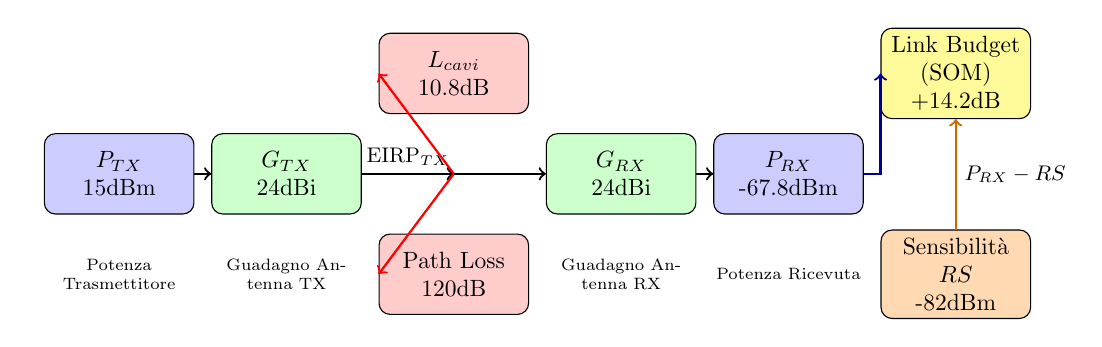
\begin{tikzpicture}[scale=0.85, every node/.style={transform shape}]
    % Definizione stili
    \tikzset{
        block/.style={rectangle, draw, fill=blue!20, 
                     minimum height=1.2cm, minimum width=2.2cm, % Aumentato minimum height
                     text centered, rounded corners, text width=2cm, align=center, text=black},
        loss/.style={rectangle, draw, fill=red!20,
                    minimum height=1.2cm, minimum width=2.2cm, % Aumentato minimum height
                    text centered, rounded corners, text width=2cm, align=center, text=black},
        gain/.style={rectangle, draw, fill=green!20,
                    minimum height=1.2cm, minimum width=2.2cm, % Aumentato minimum height
                    text centered, rounded corners, text width=2cm, align=center, text=black}
    }
    
    % Elementi del Link Budget
    \node[block] (ptx) at (0,0) {$P_{TX}$ \\
    \SI{15}{dBm}};
    \node[gain] (gtx) at (2.5,0) {$G_{TX}$ \\
    \SI{24}{dBi}};
    \node[loss] (lcavi) at (5,1.5) {$L_{\text{cavi}}$ \\
    \SI{10.8}{dB}};
    \node[loss] (lpath) at (5,-1.5) {Path Loss \\
    \SI{120}{dB}};
    \node[gain] (grx) at (7.5,0) {$G_{RX}$ \\
    \SI{24}{dBi}};
    \node[block] (prx) at (10,0) {$P_{RX}$ \\
    \SI{-67.8}{dBm}};
    
    \node[block, fill=orange!30] (rs) at (12.5, -1.5) {Sensibilità $RS$ \\
    \SI{-82}{dBm}};
    \node[gain, fill=yellow!40] (som) at (12.5, 1.5) {Link Budget (SOM) \\
    \SI{+14.2}{dB}};

    % Frecce di flusso del segnale e calcolo
    \draw[->, thick] (ptx.east) -- (gtx.west);
    \draw[->, thick] (gtx.east) -- node[above, midway, font=\small, black] {EIRP$_{TX}$} (5,0); % Punto intermedio per perdite
    \draw[->, thick, red] (5,0) -- (lcavi.west) ;
    \draw[->, thick, red] (5,0) -- (lpath.west);
    \draw[->, thick] (5,0) -- node[above, midway, font=\small, black] {} (grx.west);
    \draw[->, thick] (grx.east) -- (prx.west);
    
    % Frecce per calcolo SOM
    \draw[->, thick, blue!60!black] (prx.east) -| (som.west);
    \draw[->, thick, orange!80!black] (rs.north) -- (som.south) node[midway, right, font=\small, black] {$P_{RX} - RS$};
    
    % Etichette descrittive sotto i blocchi (opzionale, se c'è spazio)
    \node[text width=2.5cm, align=center, font=\scriptsize] at (0,-1.5) {Potenza Trasmettitore};
    \node[text width=2.5cm, align=center, font=\scriptsize] at (2.5,-1.5) {Guadagno Antenna TX};
    \node[text width=2.5cm, align=center, font=\scriptsize] at (7.5,-1.5) {Guadagno Antenna RX};
    \node[text width=2.5cm, align=center, font=\scriptsize] at (10,-1.5) {Potenza Ricevuta};

\end{tikzpicture}
\end{center}

\subsubsection{Comparazione di Scenari di Link Budget}
La tabella seguente mostra come i parametri del Link Budget cambiano in diversi scenari tipici:

\begin{table}[H]
\centering
\begin{tabular}{|l|c|c|c|}
    \hline
    \textbf{Parametro} & \textbf{Indoor} & \textbf{Outdoor} & \textbf{Long Range} \\
\hline
$P_{TX}$ & \SI{15}{dBm} & \SI{20}{dBm} & \SI{25}{dBm} \\
$G_{TX}$ & \SI{3}{dBi} & \SI{8}{dBi} & \SI{24}{dBi} \\
$L_{\text{cavi}}$ & \SI{2}{dB} & \SI{4}{dB} & \SI{8}{dB} \\
Path Loss & \SI{60}{dB} (\SI{15}{m}) & \SI{90}{dB} (\SI{150}{m}) & \SI{120}{dB} (\SI{5}{km}) \\
$G_{RX}$ & \SI{2}{dBi} & \SI{8}{dBi} & \SI{24}{dBi} \\
\hline
$P_{RX}$ & \SI{-42}{dBm} & \SI{-62}{dBm} & \SI{-55}{dBm} \\
\hline
RS & \SI{-75}{dBm} & \SI{-80}{dBm} & \SI{-85}{dBm} \\
Fade Margin & \SI{10}{dB} & \SI{15}{dB} & \SI{20}{dB} \\
\hline
\textbf{SOM} & \textbf{\SI{33}{dB}} & \textbf{\SI{18}{dB}} & \textbf{\SI{30}{dB}} \\
\textbf{Affidabile?} & \textbf{Sì} (33 > 10) & \textbf{Sì} (18 > 15) & \textbf{Sì} (30 > 20) \\
\hline
\end{tabular}
\label{tab:link_budget_scenarios}
\caption{Comparazione Scenari Link Budget (Valori Esempio)}
\end{table}

\begin{itemize}
    \item $P_{TX}$: Potenza di Trasmissione
    \item $G_{TX}$: Guadagno Antenna Trasmittente
    \item $L_{\text{cavi}}$: Perdite nei Cavi Totali
    \item $G_{RX}$: Guadagno Antenna Ricevente
    \item $P_{RX}$: Potenza Ricevuta Calcolata
    \item RS: Sensibilità del Ricevitore
    \item SOM: System Operating Margin (Link Budget)
\end{itemize}

\textbf{Descrizione degli Scenari:}
\begin{itemize}
    \item \textbf{Indoor WiFi (es. Domestico/Ufficio):}
    \begin{itemize}
        \item Distanze relativamente brevi (es. \SIrange{5}{20}{\meter}).
        \item Antenne omnidirezionali o a basso guadagno integrate nei dispositivi.
        \item Ostacoli significativi: muri, mobili, persone, che contribuiscono al Path Loss.
        \item Sensibilità del ricevitore moderata, Fade Margin per coprire variazioni interne.
    \end{itemize}
    
    \item \textbf{Outdoor Urbano (es. Hotspot Pubblico, Copertura Campus):}
    \begin{itemize}
        \item Distanze medie (es. \SIrange{50}{300}{\meter}).
        \item Antenne settoriali o omnidirezionali esterne con guadagno moderato montate su pali o edifici.
        \item Ostacoli: edifici, vegetazione, traffico. Il Path Loss è più elevato rispetto allo spazio libero.
        \item Fade Margin più elevato per far fronte a un ambiente più dinamico e variabile.
    \end{itemize}
    
    \item \textbf{Long Range Point-to-Point (PtP) (es. Ponte Radio tra Edifici/Torri):}
    \begin{itemize}
        \item Lunghe distanze (es. \SIrange{1}{20}{\kilo\meter} o più).
        \item Antenne altamente direttive (paraboliche, grid) con alto guadagno, richiedono allineamento preciso.
        \item Si punta ad avere una Line of Sight (LOS) chiara, minimizzando le ostruzioni (inclusa la Zona di Fresnel).
        \item I ricevitori possono avere sensibilità migliori (più negative). È necessario un Fade Margin consistente per garantire affidabilità su lunghe distanze e contro fenomeni atmosferici.
    \end{itemize}
\end{itemize}

\subsubsection{Visualizzazione degli Scenari di Applicazione}

\begin{center}
\begin{tikzpicture}[scale=0.65, every node/.style={transform shape}]
    % Scenario Indoor
    \begin{scope}[shift={(-7,0)}]
        \node[font=\bfseries, text width=2cm, align=center] at (0,3.5) {Indoor WiFi (Casa/Ufficio)};
        % Contesto casa/ufficio
        \draw[thick, fill=gray!10] (-2.5,-1) rectangle (2.5,2.5);
        \draw (-2.5,2.5) -- (0,3.5) -- (2.5,2.5); % Tetto semplice
        \draw[thick] (-0.5, -1) -- (-0.5, 2.5); % Muro interno
        % AP (router WiFi)
        \node[draw, fill=red!30, circle, minimum size=5mm, label={[font=\tiny, black]below:AP}] (ap_indoor) at (-1.5,0.5) {};
        % Client (laptop)
        \node[draw, fill=themeblue!40, rectangle, rounded corners=1mm, minimum width=6mm, minimum height=4mm, label={[font=\tiny, black]below:Client}] (client_indoor) at (1.5,1) {};
        % Segnale con onde che indicano ostacoli
        \draw[red!70, thick, decorate, decoration={snake, segment length=3mm, amplitude=0.5mm}] (ap_indoor) -- (client_indoor);
        \node[font=\tiny, text width=2cm, align=center] at (0, -2) {D: \SIrange{5}{20}{m}\\
        Ant: Basso Guadagno\\
        Ostacoli: Muri, Mobili};
    \end{scope}
    
    % Scenario Outdoor Urbano
    \begin{scope}[shift={(0,0)}]
        \node[font=\bfseries, text width=2.5cm, align=center] at (0,3.5) {Outdoor Urbano (Hotspot)};
        % Contesto urbano stilizzato
        \fill[gray!30] (-3,-1) rectangle (-1,1.5); % Edificio 1
        \fill[gray!40] (1,-1) rectangle (3,2);   % Edificio 2
        \draw[thick] (-3,-1) -- (3,-1); % Strada/Piazza
        % AP (antenna su palo)
        \draw[thick] (0,1.5) -- (0,2.5); % Palo
        \node[draw, fill=red!30, regular polygon, regular polygon sides=3, minimum size=7mm, label={[font=\tiny, black]above:AP Settoriale}] (ap_outdoor) at (0,2.5) {};
        % Clienti (smartphone)
        \node[draw, fill=themeblue!40, rounded corners=1mm, minimum width=3mm, minimum height=6mm, label={[font=\tiny, black]below:C1}] (c1_outdoor) at (-2,0) {};
        \node[draw, fill=themeblue!40, rounded corners=1mm, minimum width=3mm, minimum height=6mm, label={[font=\tiny, black]below:C2}] (c2_outdoor) at (0.5,-0.5) {};
        \node[draw, fill=themeblue!40, rounded corners=1mm, minimum width=3mm, minimum height=6mm, label={[font=\tiny, black]below:C3}] (c3_outdoor) at (2,0.5) {};
        % Segnali
        \draw[red!70, thick, decorate, decoration={snake, segment length=4mm, amplitude=0.4mm}] (ap_outdoor) -- (c1_outdoor);
        \draw[red!70, thick, decorate, decoration={snake, segment length=4mm, amplitude=0.4mm}] (ap_outdoor) -- (c2_outdoor);
        \draw[red!70, thick, decorate, decoration={snake, segment length=4mm, amplitude=0.4mm}] (ap_outdoor) -- (c3_outdoor);
        \node[font=\tiny, text width=2cm, align=center] at (0,-2) {D: \SIrange{50}{300}{m}\\
        Ant: Guadagno Medio\\
        Ostacoli: Edifici};
    \end{scope}
    
    % Scenario Long Range PtP
    \begin{scope}[shift={(7,0)}]
        \node[font=\bfseries, text width=2.5cm, align=center] at (0,3.5) {Long Range (Ponte Radio)};
        % Torri stilizzate
        \draw[thick, fill=gray!50] (-2.2,-1) -- (-1.8,-1) -- (-1.8,2) -- (-2.2,2) -- cycle; % Torre TX
        \draw[thick, fill=gray!50] (1.8,-1) -- (2.2,-1) -- (2.2,2) -- (1.8,2) -- cycle;   % Torre RX
        % Antenne paraboliche (semplificate)
        \draw[thick, fill=blue!30] (-1.8,1.5) ellipse (0.3cm and 0.5cm);
        \node (ant_tx_lr) at (-1.5,1.5) {};
        \draw[thick, fill=blue!30] (1.8,1.5) ellipse (0.3cm and 0.5cm);
        \node (ant_rx_lr) at (1.5,1.5) {};
        % Segnale direttivo (LOS)
        \draw[red!80, ultra thick, ->] (ant_tx_lr) -- (ant_rx_lr);
        \node[font=\tiny, red!80!black] at (0,1.8) {LOS}; 
        % Indicazione distanza
        \draw[<->, thin] (-1.8,-1.2) -- (1.8,-1.2) node[midway, below, font=\tiny] {D: \SIrange{1}{20}{\kilo\meter}};
        \node[font=\tiny, text width=2cm, align=center] at (0,-2) {Ant: Alto Guadagno\\
        LOS Critica};
    \end{scope}
\end{tikzpicture}
\end{center}

\end{document}